\section{Experiments}
\label{sec:experiments}
\subsection{Diagnosis: where the solve rate is lost}
\label{sec:diagnosis}
The diagnosis supplies the behaviours that later edits target. It is observational: every odds ratio is a within-task (Mantel--Haenszel) association. The authoring model first computed the edit-failure and calls-before-first-edit tallies. We then recomputed them from the saved trajectories with our own code (\texttt{diag\_recompute}). Every reported value reproduces, with two episodes moved between groups (Appendix~\ref{app:diag}).

\begin{itemize}
    \item \textbf{The model is inconsistent, not incapable.} Evaluation is greedy. Yet over the 13 unedited runs of batches 3--15, a single run solves 22--30 tasks, 51 different tasks are solved at least once, and 9 are solved in every run.
    \item \textbf{Failed edits go with lost episodes.} In those 13 runs (2,210 episodes), 35\% of 4,916 \texttt{edit\_file} calls fail (1,727). Episodes with no failed edit are solved 21\% of the time (318 of 1,538). Episodes with at least one failed edit are solved 4\% of the time (24 of 672). The within-task odds ratio of solving given any failed edit is 0.42 (95\% CI 0.23--0.74). If we also count the 165 edit calls that the harness rejected before running, 38.5\% fail and the odds ratio is 0.44.
    \item \textbf{Long exploration loses episodes.} Over the same 2,210 episodes, 17\% of episodes make 8 or more calls before the first file edit. Within task, these episodes solve far less than the task's other episodes (odds ratio 0.12, 95\% CI 0.04--0.38). We bin the 6 episodes that never edit a file by their total calls; three fall in 8+, all unsolved. On the 2,204 episodes with at least one file edit, the 8+ odds ratio is unchanged (0.12, CI 0.04--0.37; \texttt{dr\_fix/m4\_8plus\_edited\_only.py}). Episodes that never edit therefore do not drive it. The other bins have intervals that include 1 (0--2 calls 0.76, CI 0.39--1.48; 3--4 calls 1.42, 0.86--2.35; 5--7 calls 1.72, 0.97--3.06; Figure~\ref{fig:invu}). Raw solve rates are highest for 0--2 calls, because the model edits easy tasks quickly. Each bin draws on 19 to 36 informative tasks, because most tasks are never solved.
    \item \textbf{Reading before editing.} On the three unedited runs of batches 3--5 (510 episodes, 7 informative tasks), reading a file before the first edit shows no association with solving (odds ratio 1.0). Pooled over all 2,720 episodes of those batches (the 16 runs of the 170 tasks in the scripted per-episode file, edited arms included; the other runs of those batches are not in it), episodes that read first were solved more often (371 of 2,259 against 38 of 461; odds ratio 3.1, $z = 4.5$, 51 tasks with both outcomes and both conditions). This pooled association comes from the edited arms. Claude's later tally found no monotone benefit of longer exploration (Appendix~\ref{app:diag}).
\end{itemize}

\begin{figure}[t]
\begin{center}
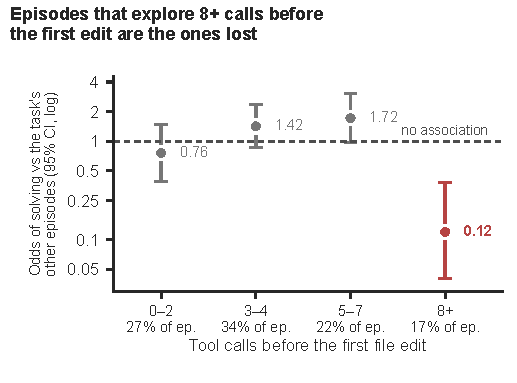
\includegraphics[width=0.5\linewidth]{figures/fig5_invu.pdf}
\end{center}
\caption{\textbf{Long exploration before the first edit is where episodes are lost.} Within-task Mantel--Haenszel odds ratio of solving for episodes in each bin of tool calls before the first file edit, against the task's other episodes; 13 unedited runs, 2,210 episodes; 95\% Robins--Breslow--Greenland intervals, log scale. Only the 8+ bin (red) excludes 1. The 6 episodes with no file edit are binned by their total calls; without them the 8+ odds ratio is 0.12 (0.04--0.37). Observational.}
\label{fig:invu}
\end{figure}

\subsection{Edits control decisions}
\label{sec:control}
\textbf{Claim tested:} an edit moves its targeted decision monotonically with its strength, and a matched random control of the same size does not.

\textbf{Setting.} For each edit, we regenerate held-out logged decisions once, greedily, and count the targeted decision. We do this under the unedited model, the edit at three strengths, and a matched random control. Intervals are Wilson 95\% intervals for proportions. We write the submit-sooner edit on the wave-5 RL adapter. Its submit-versus-keep-testing direction has held-out AUC 0.72--0.75 at the three written layers. We write the think-briefly and explore-more edits on the base model. This replay covers the always-on edits. For the gated edits of \S\ref{sec:arena}, we measured static per-position shifts (below) and teacher-forced comparisons (Appendix~\ref{app:hook}).

\begin{figure}[t]
\begin{center}
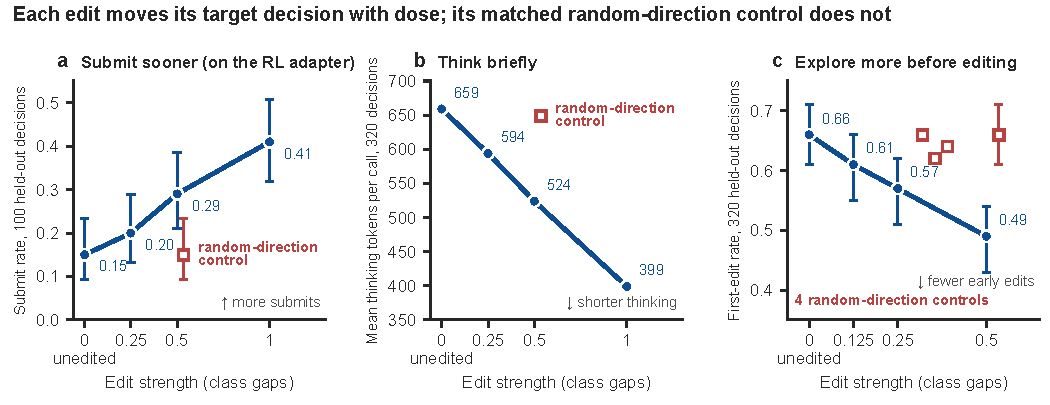
\includegraphics[width=1.0\linewidth]{figures/fig2_dose.pdf}
\end{center}
\caption{\textbf{Edits control decisions with dose; matched controls do not.} Replay of held-out logged decisions under the unedited model (strength 0), the edit at three strengths (blue) and matched random-direction controls (red squares, same neurons and norm). (a) Submit rate over $n = 100$ decisions, edit written on the RL adapter. (b) Mean thinking tokens per call over $n = 320$ decisions (means only; one control seed, matched to strength 0.5). (c) Rate at which the next call makes the episode's first edit, $n = 320$; four control adapters, one matched to strength 0.5 and three seeds matched to 0.25. Bars: Wilson 95\% intervals.}
\label{fig:dose}
\end{figure}

\textbf{Result.} Figure~\ref{fig:dose} and Table~\ref{tab:dose} (Appendix~\ref{app:params}) show a monotone dose-response for all three edits. The submit rate rises from 0.15 to 0.41; the control gives 0.15. Thinking tokens fall from 659 to 399; the control gives 649. The rate at which the next call makes the first edit falls from 0.66 to 0.49. The four control adapters give 0.66, 0.62, 0.64 and 0.66. The unedited rate was 0.64 to 0.66 in three separate replay runs, so replay noise is about 0.02. At the lowest strength (0.125; rate 0.606), the edit does not separate from the controls; one control seed gives 0.616. The effect carries from single decisions to whole episodes. The submit-sooner edit lowers mean tool calls per episode from 20.8 to 14.2 at strength 0.5 and to 8.8 at strength 1.0. Its 0.5-matched control gives 19.8 (one agent run per arm).

\textbf{Off-target effects.} Each edit also moves other statistics. Think-briefly at strength 1.0 lowers the first-edit rate from 0.64 to 0.52. At strength 0.5 it gives 0.60, the same as its 0.5-matched random control (0.60). Submit-sooner at strength 1.0 lowers thinking tokens per call from 282 to 167 (strength 0.5: 238; its 0.5-matched control: 288).

\textbf{Locality of gated edits.} The gated edits of \S\ref{sec:arena} allow a per-position check. We compute it from the stored bf16 tensors on held-out positions. Claude's before-first-edit gate reads its condition with held-out AUC 0.993--0.996. It fires on 85--88\% of positions before the first edit and on 1.2--1.4\% of its OFF positions (positions after the first edit that were in its fit). The shift along the explore direction is $-0.22$ to $-0.32$ class gaps before the first edit and 0.000 at decision positions after it. At prompt positions after the first edit, which were not in its fit, the shift is $-0.19$ to $-0.21$ class gaps (early-calls gate: $-0.08$ to $-0.12$). The gate thus also acts on these prompt positions. Appendix~\ref{app:gated} gives the other gates.

\textbf{Episode cost.} Submit-sooner shortens episodes by design. The explore-more edits do not reduce episode cost relative to the unedited model (Appendix~\ref{app:negative}, Table~\ref{tab:cost}).

\subsection{Always-on explore-more on development tasks}
\label{sec:devgain}
\textbf{Claim tested:} writing ``explore more before editing'' at every position raises solved development tasks at low strength and lowers them at high strength.

\textbf{Setting.} Batches 3--15 each ran eight to eleven arms, the unedited model included (schedule in Appendix~\ref{app:schedule}). We compare every edit with the unedited model served alongside it in the same batch. In batches 3--5, we compare edits written on the RL adapter with that adapter (Appendix~\ref{app:repro}). Twelve of the 13 batches have an explore-more arm. We chose strengths on these tasks and later pre-registered strength 0.25 for the held-out test. The pool of strengths 0.125--0.5 is a post hoc summary. ``Gained / lost'' counts tasks that the arm solves and the unedited model of the same batch does not, and the reverse, summed over runs.

\begin{table}[t]
\caption{Always-on explore-more on the base model, 170 development tasks. $\Delta$ is the mean difference in solved tasks against the unedited model of the same batch, with a 95\% $t$ CI and two-sided paired $t$ test. For the edit rows the unit is the run; for the control row the 14 runs are first averaged within each of their 7 batches ($n = 7$); its Mean is the average of these batch means (25.8; the mean over the 14 runs is 25.6). ``Unedited, same batches'' is the mean of the unedited model over the batches of that row. The pooled row averages the 0.125--0.5 arms within each of 12 batches (post hoc). In batches 3--5 the base-model arms and the RL-adapter arms ran as two separate groups; every row here uses base-model arms and the unedited arm of the same group. Rows with different strengths come partly from different batches, so the within-batch comparison is the one in batches 6, 7 and 10 given in the text.}
\label{tab:explore}
\centering
\footnotesize
\setlength{\tabcolsep}{3.5pt}
\resizebox{\linewidth}{!}{\begin{tabular}{lrlrrrlrr}
\toprule
Arm & Runs & Solved per run \up & Mean \up & Unedited, same batches & $\Delta$ \up & 95\% CI & $p$ & Gained / lost \\
\midrule
Unedited model & 13 & 22--30 & 26.3 & & & & & \\
Explore-more 0.125 & 4 & 31, 30, 28, 33 & 30.5 & 26.0 & $+4.5$ & [$-0.3$, $+9.3$] & 0.058 & 40 / 22 \\
Explore-more 0.25 & 7 & 32, 29, 30, 31, 29, 26, 27 & 29.1 & 25.1 & $+4.0$ & [$+0.3$, $+7.7$] & 0.040 & 75 / 47 \\
Explore-more 0.5 & 10 & 28, 31, 33, 30, 26, 32, 30, 24, 28, 27 & 28.9 & 26.2 & $+2.7$ & [$-0.3$, $+5.7$] & 0.074 & 98 / 71 \\
Explore-more 1.0 & 1 & 18 & 18.0 & 24.0 & $-6.0$ & & & 8 / 14 \\
Pooled 0.125--0.5 & 12 batches & & 28.8 & 26.2 & $+2.7$ & [$+0.3$, $+5.0$] & 0.030 & \\
Matched random controls & 14 & 23--28 & 25.8 & 25.9 & $-0.04$ & [$-3.1$, $+3.0$] & 0.98 & 116 / 117 \\
\bottomrule
\end{tabular}}
\end{table}

\textbf{Result.} In Table~\ref{tab:explore} (per-run counts: Figure~\ref{fig:solve}, Appendix~\ref{app:negative}), the gain shrinks as strength grows from 0.125 to 0.5. These rows cover different batches. In the three batches that ran all three strengths together (6, 7 and 10), the means are 29.7, 30.0 and 31.0 for strengths 0.125, 0.25 and 0.5, against 25.7 for the unedited model: within a batch, the gain is flat across this range. The single run at strength 1.0 is 6 tasks below its unedited model. We average the edit arms at strengths 0.125--0.5 within each batch; this pooled quantity is distinct from the strength-0.5 row, which has the same $\Delta$. The pooled edit exceeds the unedited model by 2.7 tasks over 12 batches (95\% CI $+0.3$ to $+5.0$, $p = 0.03$; higher in 9 batches, sign test $p = 0.15$). It exceeds the mean of the random controls by 3.6 tasks in the 7 batches that contain both (CI $+2.2$ to $+5.1$, $p < 0.001$; higher in 7 of 7, sign test $p = 0.016$). The controls do not differ detectably from the unedited model in those batches ($-0.04$ tasks, 95\% CI $-3.1$ to $+3.0$). The pre-registered strength 0.25 alone exceeds the controls by 3.7 over 6 batches (CI $+2.1$ to $+5.3$, $p = 0.002$). It exceeds its own 0.25-matched controls by 3.3 over the 5 batches that contain them (CI $+1.3$ to $+5.2$, $p = 0.010$; \texttt{dr\_fix/exp\_checks.py}). The reversed sign (``edit sooner'') solved 12 at strength 1.0 and 22 at strength 0.5, against 28 for the unedited model in one batch.

\textbf{Replication trend and coverage.} The gain was $+4.3$ in the first six batches with an edit arm (4--9; $p = 0.07$) and $+1.1$ in the last six (10--15; CI $-1.2$ to $+3.4$, $p = 0.27$). Of the 170 tasks, 90 were never solved in any of the 109 complete runs of batches 3--15. In the 96 runs on the base model (excluding the 13 runs on the RL adapter), 94 were never solved. The edit therefore acts on reliability on tasks that the model can already solve.
